
\chapter{Format danych wejściowych}

Problem układania planu zajęć jest popularny w świecie naukowym. Dostępnych jest wiele rozwiązań tego problemu i ciągle powstają nowe. Jednak, by móc porównać ze sobą algorytmy rozwiązywania problemu, konieczne jest operowanie na tych samych danych testowych. Z tego powodu badacze uzgodnili jednolity format danych wejściowych o nazwie XHSTT i stworzyli bazę danych wraz z przykładowymi rozwiązaniami \cite{Database}. Dane te zapisane są za pomocą języka XML. Format XHSTT jest skomplikowany, dlatego w niniejszej pracy poświęcono cały rozdział na jego opisanie \cite{XHSTT}. 

\section{Budowa archiwum}

\begin{figure}
	\centering
	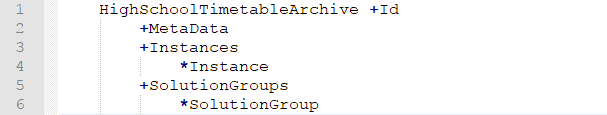
\includegraphics {szablonXHSTT}
	\caption{Szablon dokumentu w archiwum XHSTT.}
	\label{fig: szablonXhstt}
\end{figure}
Archiwum jest kolekcją instancji zawierających dane dla problemu układania planu zajęć, razem z potencjalnymi grupami rozwiązaniami. Każda grupa rozwiązań zawiera rozwiązania dla jednej instancji z archiwum. Ogólny szablon dokumentu przedstawiono na rysunku 4.1. W tym szablonie, słowa znajdujące się w tym samym wierszu oznaczają, że pierwsze  słowo jest nazwą kategorii, a kolejne słowa to jej atrybuty. Słowa umieszczone poniżej w zagłębieniach to nazwy podkategorii. Znak + przed nazwą oznacza, że kategoria lub atrybut jest opcjonalny. Znak * oznacza, że dana kategoria może wystąpić zero lub więcej razy. Przykład dokumentu w formacie XML zaprezentowano na rysunku 4.2.

\begin{figure}
	\centering
	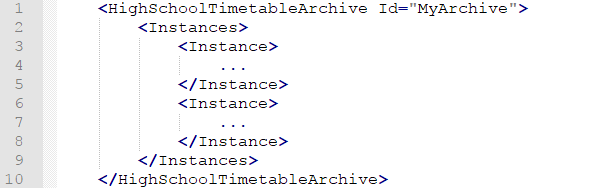
\includegraphics {szablonXHSTTprzyklad}
	\caption{Przykład archiwum w języku XML.}
	\label{fig: Xhsttprzyklad}
\end{figure}

Opcjonalna kategoria \textit{Metadata} zawiera podstawowe informacje na temat archiwum, takie jak nazwa archiwum, autor, data powstania, opis oraz uwagi.

\section{Instancje}

Instancja jest to pojedynczy zestaw danych dla danego problemu układania planu zajęć, najczęściej dla pojedynczej szkoły i konkretnego roku (lub semestru). Postać instancji zaprezentowano na rysunku 4.3. Wiele kategorii ma atrybut \textit{Id}, który służy do odwoływania się do danej kategorii w dalszej części archiwum.

\begin{figure}
	\centering
	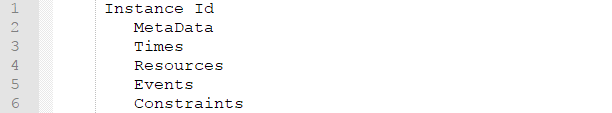
\includegraphics {skladniaSzablon}
	\caption{Szablon pojedynczej instancji.}
	\label{fig: skladniaSzablon}
\end{figure}

\section{Okna czasowe}

W formacie XHSTT przyjęto tylko prosty model czasu, w którym czas podzielony jest na równe interwały zwane oknami czasowymi. Kategoria \textit{Times} (rysunek 4.4) służy do definiowania okien. Podkategoria \textit{TimeGroups} definiuje różne grupy czasowe, takie jak dni, tygodnie oraz okresy w ciągu dnia. Podkategoria \textit{Time} zawiera definicje okna czasowego, w której każde okno oprócz nazwy może mieć przypisany konkretny tydzień, dzień i inne grupy czasowe. Przykład w języku XML znajduje się na rysunku 4.5. Przedstawia on czwarte okno czasowe w poniedziałek.

\begin{figure}
	\centering
	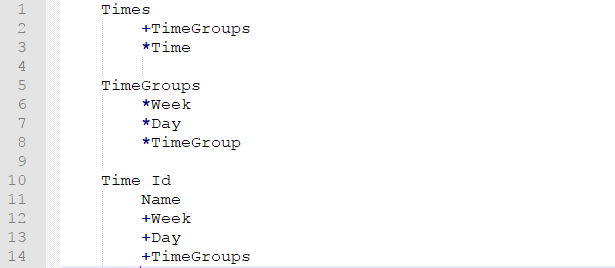
\includegraphics {skladniaTimes}
	\caption{Składnia kategorii \textit{Times}.}
	\label{fig: skladniaTimes}
\end{figure}

\begin{figure}
	\centering
	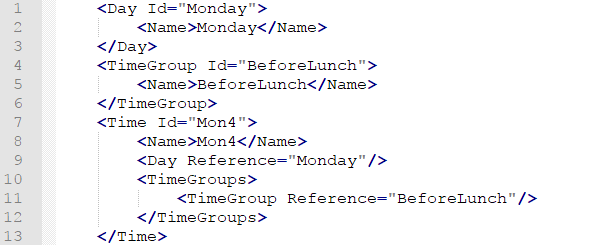
\includegraphics {timesPrzyklad}
	\caption{Przykład deklaracji czwartego okna czasowego w poniedziałek.}
	\label{fig: timesPrzyklad}
\end{figure}

\section{Zasoby}

Zasoby są to wszystkie elementy przypisane do zdarzeń. Do zasobów najczęściej zaliczamy nauczycieli, sale i grupy uczniów, ale dodatkowo format XHSTT umożliwia dowolne definiowanie zasobów. W skład kategorii \textit{Resources} (rysunek 4.6) wchodzą również grupy i typy zasobów. Typ zasobów to np. nauczyciel, sala, grupa. Grupy zasobów gromadzą zasoby jednego typu, np. nauczyciele języka polskiego.Na rysunku 4.7 zaprezentowano przykładową deklarację sali komputerowej.

\begin{figure}
	\centering
	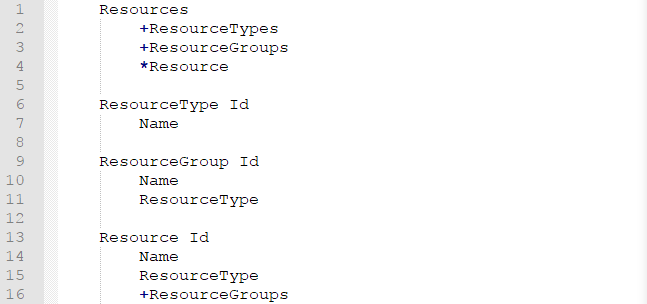
\includegraphics {resourcesSkladnia}
	\caption{Składnia kategorii \textit{Resources}.}
	\label{fig: resourcesSkladnia}
\end{figure}

\begin{figure}
	\centering
	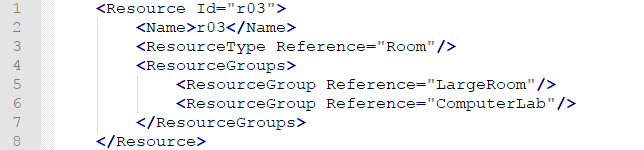
\includegraphics {resourcesPrzyklad}
	\caption{Przykład deklaracji zasobu w postaci sali komputerowej.}
	\label{fig: resourcesPrzyklad}
\end{figure}

\section{Zdarzenia}

Zdarzenia określone są jako spotkanie między zasobami, czyli w uproszczeniu są to zajęcia odbywające się w danej sali, z danym nauczycielem i grupą studentów. Przed zdarzeniami zdefiniowane mogą być ich grupy, takie jak np. zajęcia z języka obcego. Zdarzenia zawierają atrybuty określające czas trwania oraz termin odbycia zajęć. Termin odbywania zajęć może być przypisany wcześniej lub może być pozostawiony pusty, w celu przypisania go przez algorytm układający plan zajęć. Dodatkowo, zdarzenia mają parametr określający kolor zajęć wyświetlany na ułożonym planie. Składnia kategorii \textit{Events} zaprezentowana jest na rysunku 4.8, a na rysunku 4.9 pokazano przykładową deklarację zajęć z języka angielskiego.

\begin{figure}
	\centering
	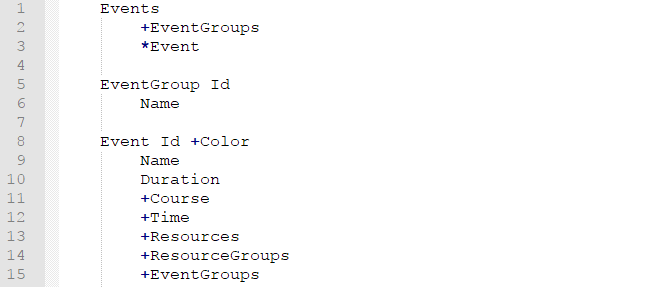
\includegraphics {eventsSkladnia}
	\caption{Składnia kategorii \textit{Events}.}
	\label{fig: eventsSkladniakladnia}
\end{figure}

\begin{figure}
	\centering
	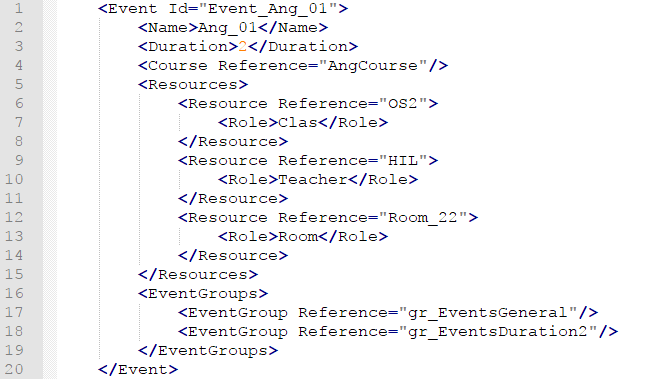
\includegraphics {eventsPrzyklad}
	\caption{Przykład deklaracji zajęć z języka angielskiego.}
	\label{fig: eventsPrzyklad}
\end{figure}

\section{Ograniczenia}

Format XHSTT umożliwia definiowanie wielu ograniczeń dotyczących planu zajęć. Wszystkie ograniczenia opisane są szczegółowo na stronie internetowej \cite{ograniczenia}. W niniejszej pracy zostały opisane tylko te, które są uwzględnione w wykonanej implementacji. Ogólna składnia ograniczenia przedstawiona jest na rysunku 4.10. Każde z ograniczeń ma zdefiniowaną wagę oraz sposób wyliczania funkcji kosztu (liniowa, kwadratowa itp.). Każde ograniczenie może być twarde lub miękkie w zależności od parametru \textit{Required}.

\begin{figure}
	\centering
	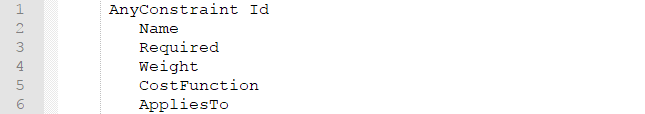
\includegraphics {ograniczeniaSkladnia}
	\caption{Składnia kategorii \textit{Constraints}.}
	\label{fig: ograniczeniaSkladnia}
\end{figure}

\begin{itemize}
	\item Przypisany czas - Ograniczenie \textit{Assign time constraints} mówi, że każde zdarzenie musi mieć przypisany czas, oraz definiuje koszt złamania tego ograniczenia. Dane ograniczenie może być przypisane do wszystkich wydarzeń, lub tylko do wybranych grup zdarzeń. Przykład przedstawiono na rysunku 4.11.
	
	\item Unikanie konfliktów - Ograniczenie \textit{Avoid clashes constraints} określa, czy dane zasoby mogą być dzielone. To znaczy, czy nie są one przypisane do dwóch lub więcej zdarzeń odbywających się w tym samym czasie. Jest to ograniczenie często stosowane, jednak mogą zdarzyć się przypadki, w których układający dopuszcza odbywanie się dwóch zajęć w jednej sali jednocześnie (np. zajęcia wychowania fizycznego).
	
	\item Podział zdarzeń - Ograniczenie \textit{Split events constraints} określa, czy zdarzenia o długości dłuższej niż jeden mogą zostać podzielone i rozłożone na kilka dni. Ograniczenie to pozwala definiować minimalne i maksymalne długości bloków danego zdarzenia.
	
	\item Limit bezczynności - Ograniczenie \textit{Limit idle times constraints} określa, czy mogą występować, i jak długie mogą być przerwy między zajęciami. Ograniczenie określa, czy między dwoma zajęciami jednego dnia może wystąpić jedno lub więcej nieprzypisanych okien czasowych.
\end{itemize}

\begin{figure}
	\centering
	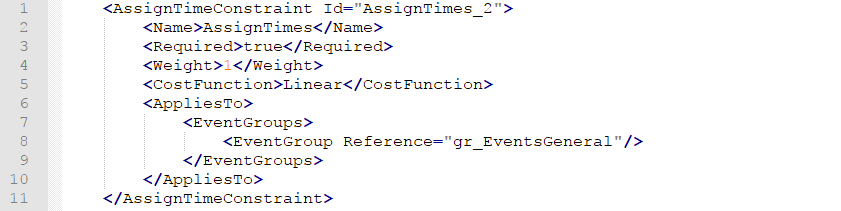
\includegraphics {ograniczeniaPrzyklad}
	\caption{Przykład ograniczenia \textit{Assign time constraints}.}
	\label{fig: ograniczeniaPrzyklad}
\end{figure}